\newpage

\subsection{Issuance Case Study}

\noindent In this section we illustrate how Havven's incentives encourage havven holders to
maintain stability.

\noindent In \ref{subsubsec:practicalissuance}, we first present a simplified example the practical issuance
dynamics for a havven holder, Bob, if he targets \(C_{opt}\). In the second part, \ref{subsubsec:coptimality},
we examine the optimality of following this strategy with a more sophisticated model
of the mechanism as a two-player game. \\

\noindent It should be noted that these are simply illustrative examples to give the 
reader a feel for the nature of the system's issuance dynamics. This
section is partly an adaptation of the calibrated analysis results presented
in much greater depth in as part of the economic analysis of Havven performed by
\href{http://cryptecon.org/}{\textcolor{blue}{cryptecon}}, which can be found in
its entirety \href{https://havven.io/uploads/havven_cryptecon_report_may_2018.pdf}{\textcolor{blue}{here}}. \\

\noindent The cryptecon investigation concluded that the Havven system
generally stabilises the nomin price at \$1, but most of the supporting
apparatus has been omitted in this white paper. Therefore, an interested reader should
consult that reference for further details and an explanation of the assumptions
which underly its results. \\

\noindent Throughout this section we will assume implementation upon Ethereuem, therefore
in this example, the system will buy and sell nomins in exchange for ether, but this could be 
substituted with any asset tradeable in a decentralised way. \\

\newpage
\subsubsection{Practical Issuance Dynamics}
\label{subsubsec:practicalissuance}

\noindent \textbf{Initial Conditions} \\

\noindent Bob decides to purchase 100 havvens at \$1 each.
The system is in price equilibrium, with the global collateralisation
ratio \(C\) equal to the optimal collateralisation ratio
\(C_{opt}\). We will denote Bob's personal \(H\) and \(C_i\) with
\(H_{bob}\) and \(C_{bob}\). The initial conditions are then as follows:

\begin{align*}
    C_{max} &= 0.5 & C_{opt} &= 0.4 & C &= 0.4 \\
    P_n &= 1 & P_h &= 1 & H_{bob} &= 100 \\
\end{align*}

\noindent The internal parameters of \(C_{opt}\) and \(C_{max}\), as described in
section~\ref{subsec:collatratio}, will remain constant throughout the example:
\begin{align*}
    \sigma &= 50 & \psi &= 3 & a&= 1.25
\end{align*}

\noindent Initially, Bob's wallet contains only free havvens, but he wants to
earn the maximum possible fees, so he issues nomins up to \(C_{opt}\).
The system generates 40 nomins and escrows 80 of his havvens,
locking \$80 worth of value in the system. The nomins are sold for \$40 worth
of ether and the proceeds are transferred to Bob's account.

%\begin{figure}[h!]
%    \centering
%    \begin{subfigure}{.5\textwidth}
%        \centering
%        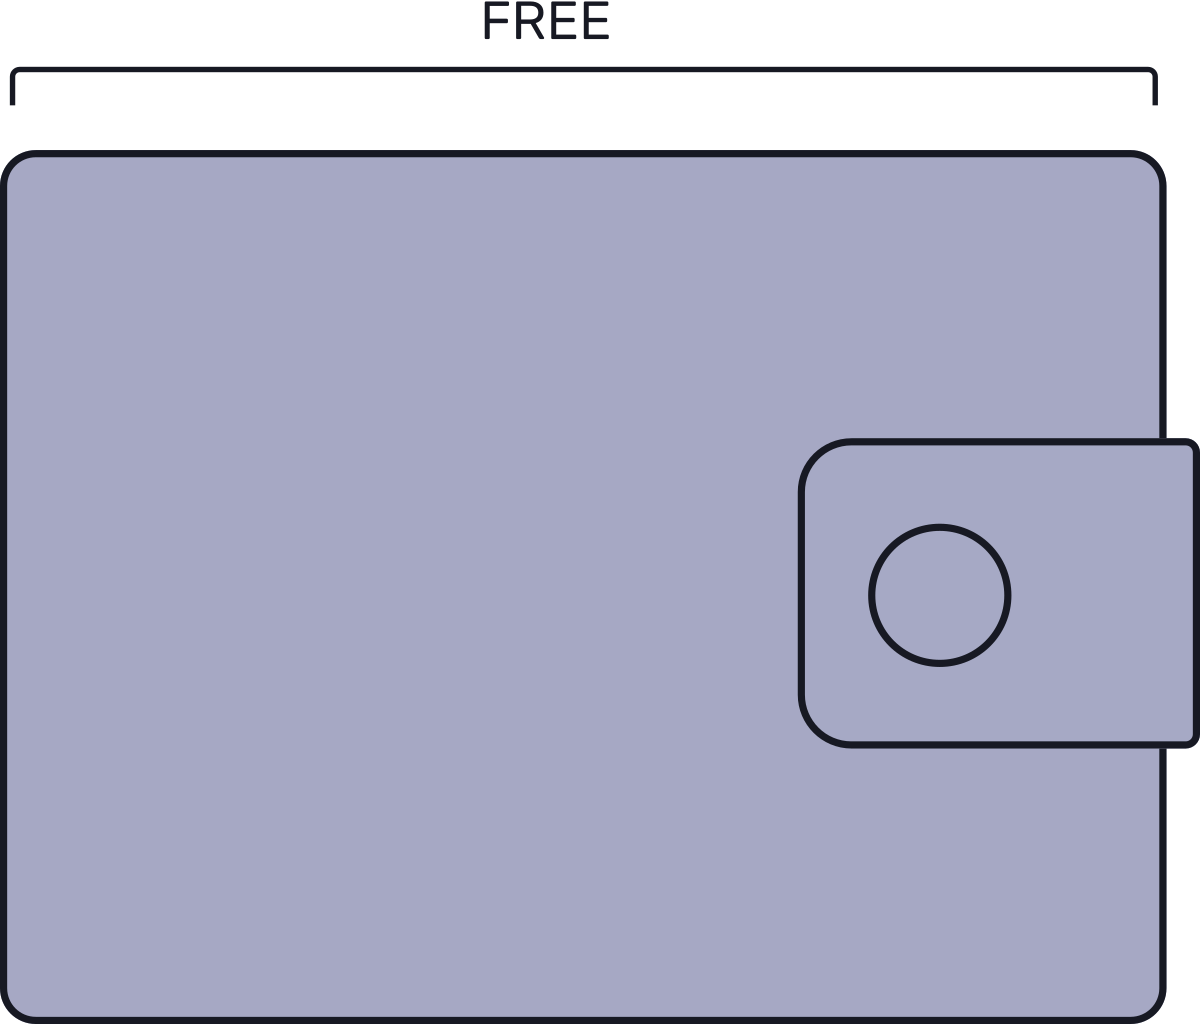
\includegraphics[width=0.60\textwidth]{img/wallet}
%    \end{subfigure}%
%    \begin{subfigure}{.5\textwidth}
%        \centering
%        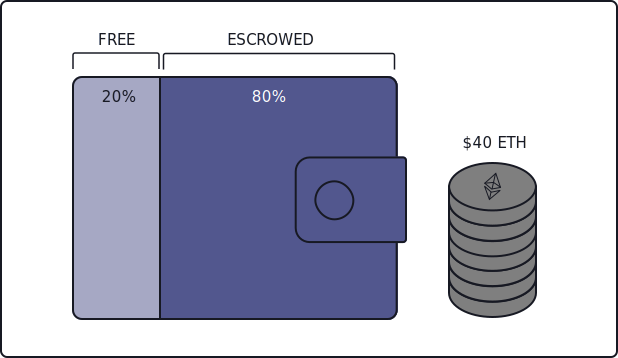
\includegraphics[width=0.80\textwidth]{img/escrowed}
%    \end{subfigure}
%\end{figure}

\begin{figure}[h!]
    \centering
    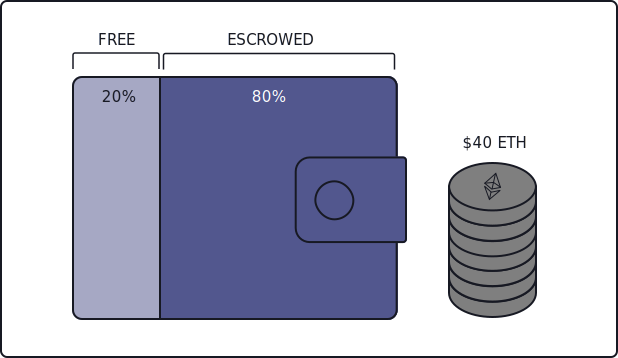
\includegraphics[width=0.40\textwidth]{img/escrowed}
\end{figure}

\vspace{2mm}

\noindent We now proceed to examine the respective consequences for Bob of nomin and havven
price shocks.

\newpage
\noindent \textbf{Nomin Price Shock} \\

\noindent This example shows how the system incentivises havven holders
to correct instability in the nomin price.

\begin{enumerate}
    \item{As a consequence of reduced demand in decentralised trading markets,
          the nomin price \(P_n\) drops to \$0.90. The system needs to incentivise havven
          holders to reduce the supply of nomins so that the price returns to \$1.00.
    }
    \item{First, consider that both \(C\) and \(C_{bob}\) have decreased to 0.36.
          Since the nomin price has changed, \(C_{opt}\) is recalculated to 0.342, which
          is smaller than both \(C_{bob}\) and \(C\). Consequently, \(C_{max}\) also changes
          to 0.4275. This increases the percentage of Bob's havvens that are locked.
    }

    \begin{figure}[h!]
        \centering
        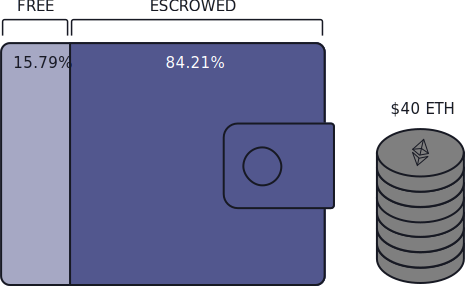
\includegraphics[width=0.4\textwidth]{img/pn_drop}
    \end{figure}

    \item{Bob now has a higher dollar value of locked havvens and \(C_{bob} > C_{opt}\).
          This means that he is no longer receiving the maximum fee rate
          \(\phi_{base}\). In order to return to \(\phi_{base}\) he must lower
          \(C_{bob}\) back to \(C_{opt}\) by burning some nomins. He needs to work out how
          many to burn.
    }

    \item{He should burn 2 nomins so that he has 38 total issued, which will cost
          \$1.80. When the system completes this process, his locked havvens will
          reduce back to 80. In addition, \(C_{bob}\) is equal to \(C_{opt}\) at 0.342,
          which means he is once again receiving the maximum fee rate.
    }
    \begin{figure}[h!]
    \centering
        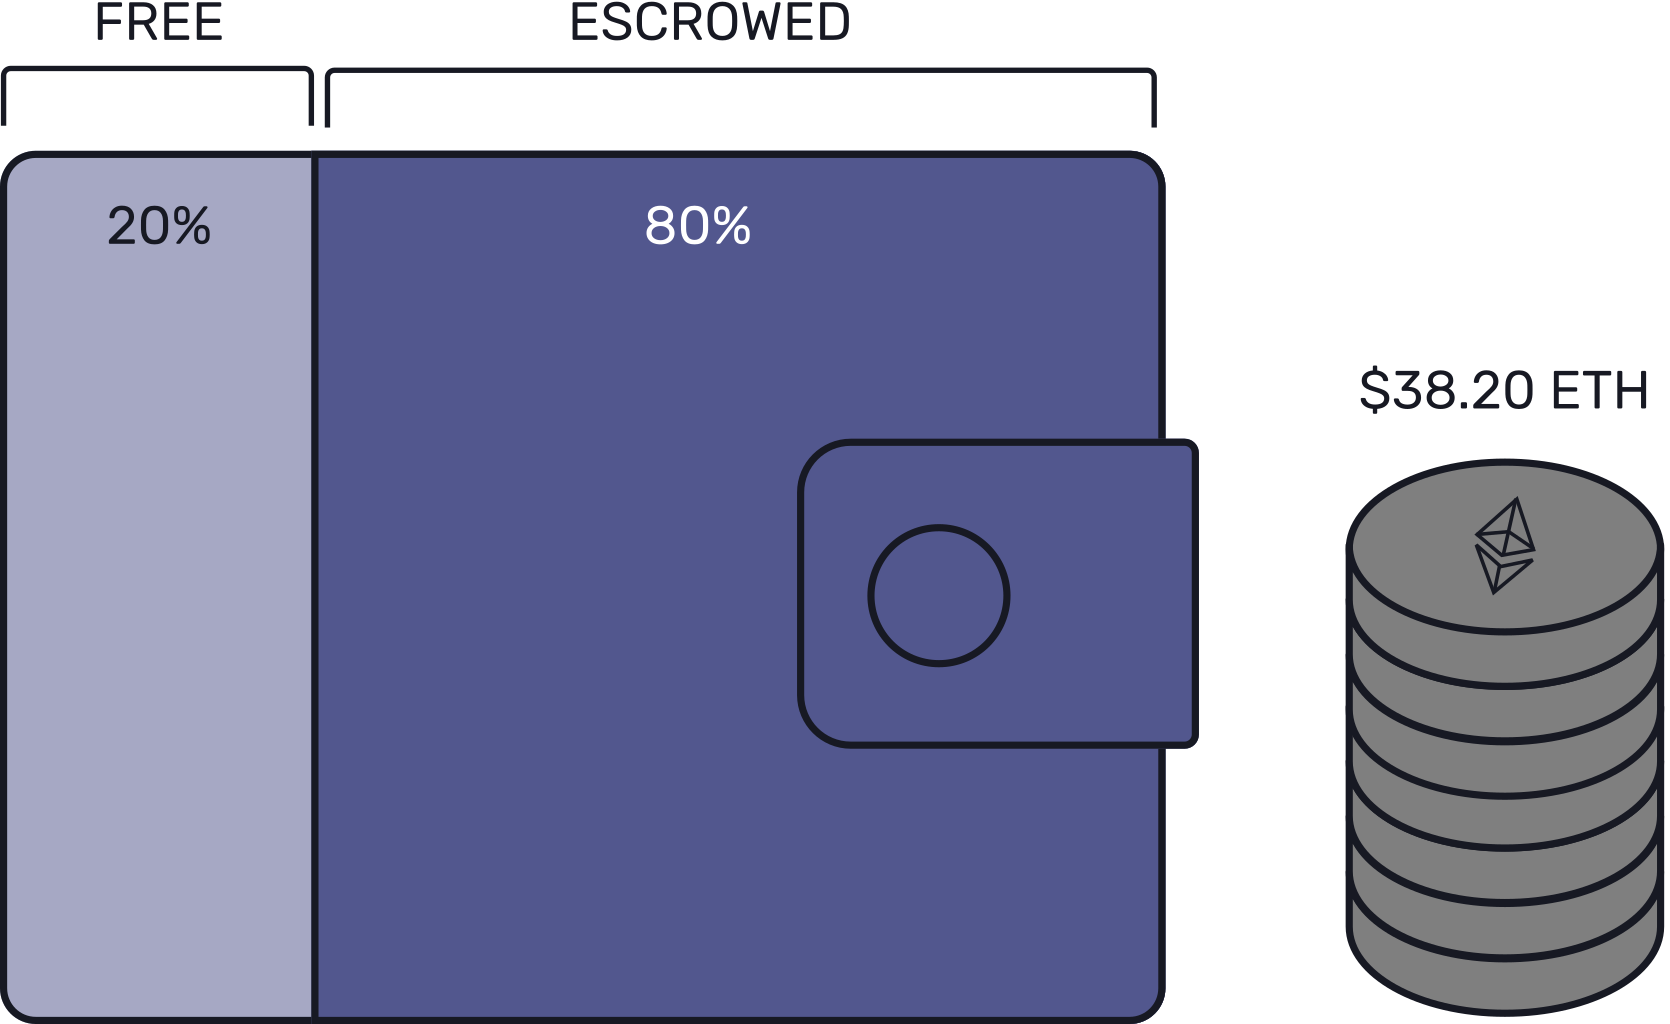
\includegraphics[width=0.4\textwidth]{img/post_burn}
    \end{figure}

    \item{Bob has taken the correct actions to raise the low nomin price. By
          electing to burn nomins, the system performed a limit buy order on his
          behalf, putting upward pressure on the nomin price. As compensation for doing
          so, he is rewarded with the optimal fee rate \(\phi_{base}\).
    }
\end{enumerate}


\newpage
\noindent \textbf{Havven Price Shock (Market Price)} \\

\noindent This example illustrates how the system maintains the dollar value of the underlying
collateral by adjusting the quantity of a user's escrowed havvens when the
havven price changes. We will use the same initial conditions as in the previous example.

\begin{enumerate}
    \item{As before, Bob elects to issue up to \(C_{opt}\) in order to maximise fees.}
    \begin{figure}[h!]
        \centering
        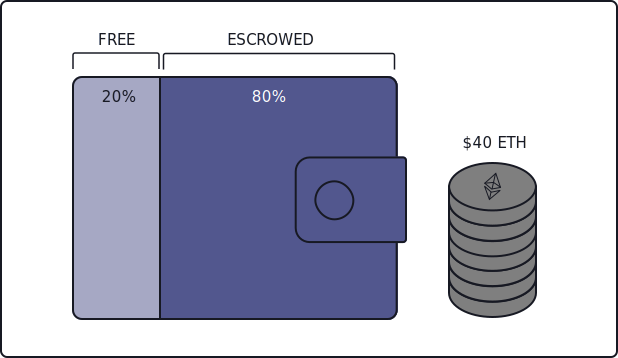
\includegraphics[width=0.4\textwidth]{img/escrowed}
    \end{figure}

    \item{The havven price \(P_h\) drops to \$0.90, which means the value of
          Bob's wallet has decreased to \$90. Both \(C\) and \(C_{bob}\) have increased to
          0.44. Since the nomin price has not changed, the system does not need to
          incentivise issuance or burning. This is reflected in the new value of
          \(C_{opt}\), which changes to 0.44, matching \(C\) and \(C_{bob}\).
    }

    \item{However, the system needs to escrow more of Bob's havvens to
          maintain the dollar value of the locked collateral. The system has now
          locked around 89\% of Bob's havvens, to maintain \$80 of locked
          collateral.
    }

    \begin{figure}[h!]
        \centering
        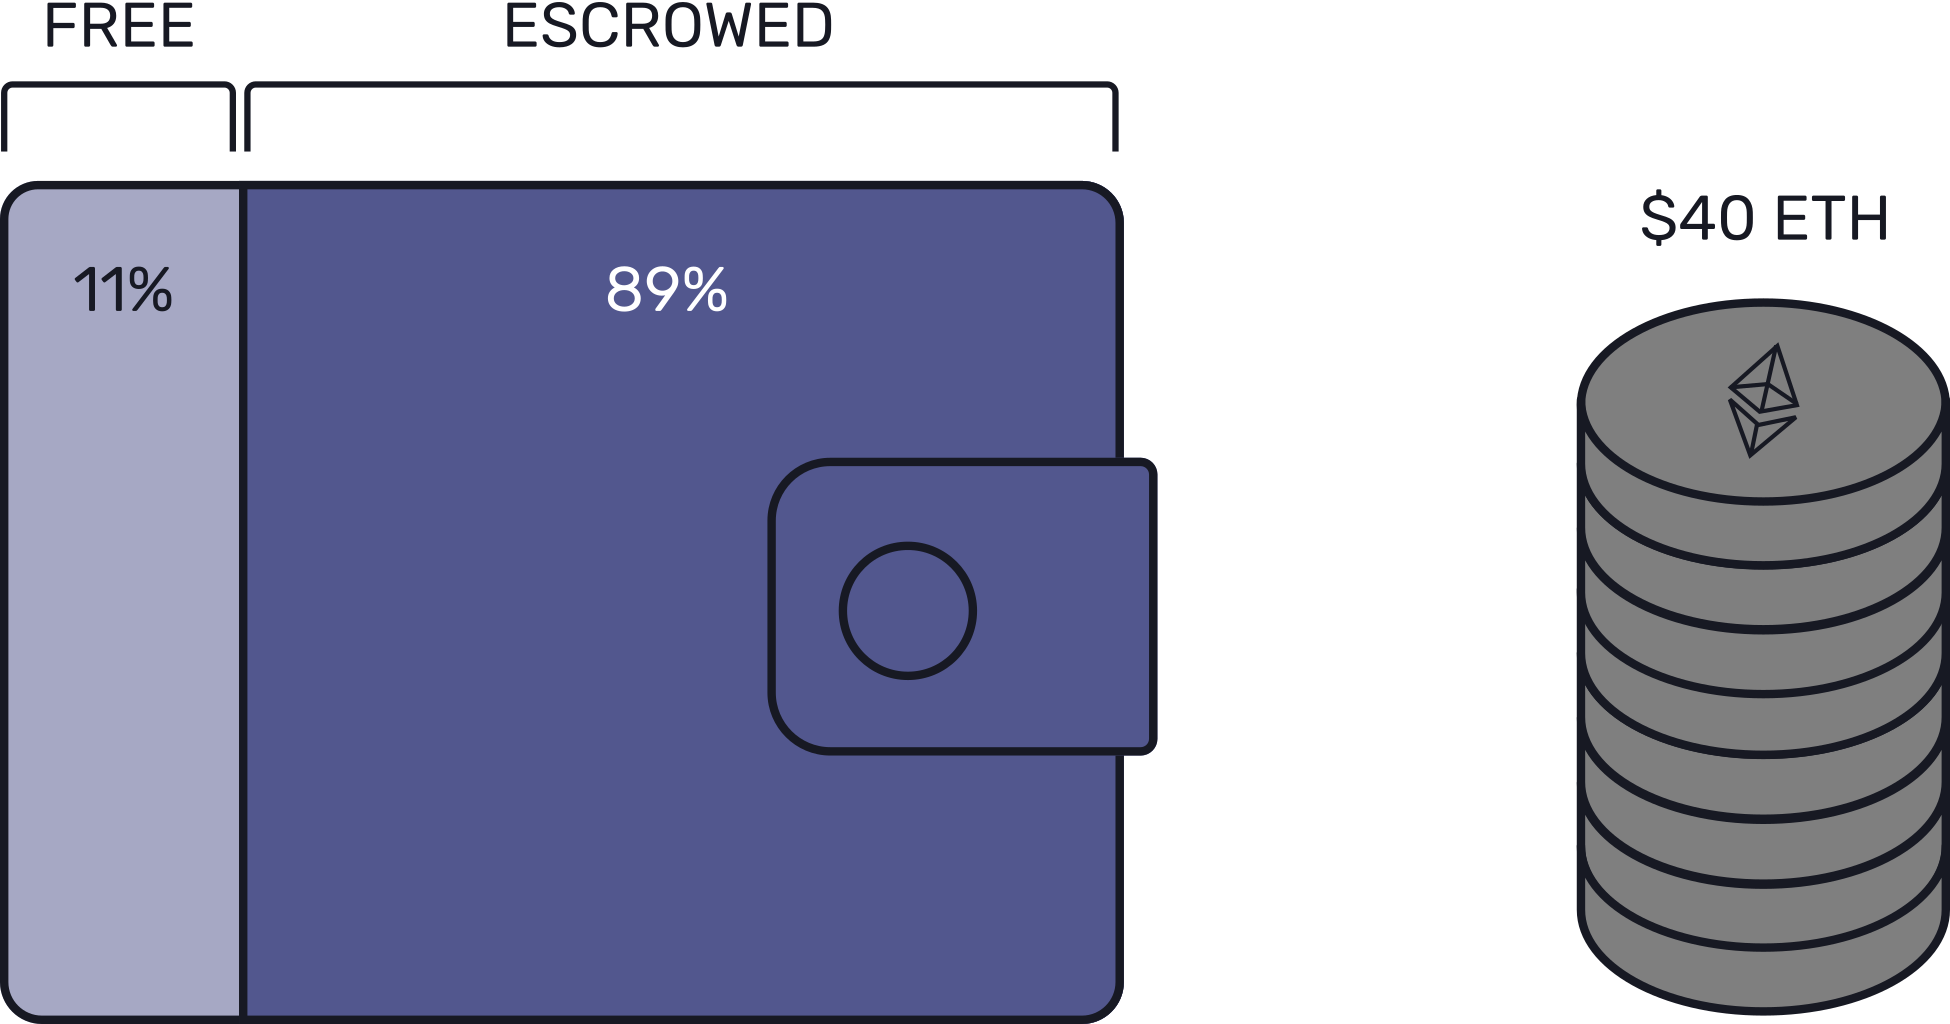
\includegraphics[width=0.5\textwidth]{img/ph_drop}
    \end{figure}
\end{enumerate} 


\newpage
\subsubsection{Optimality of Targeting \(C_{opt}\)}
\label{subsubsec:coptimality}

\noindent We will now examine the correct action for players to respond to changes in the
nomin price. The game begins in an equilibrium condition, with all players holding issuance
levels matching the optimal level. \\

\noindent For simplicity, we consider a system which has only two havven holders. We lose no generality
here, as a collection of actors behaving together can be considered as one agent. The sets of agents 
we consider are those those havven holders who do and do not respond to nomin price shocks by
matching their aggregated \(C_i\) to  \(C_{opt}\) as it changes, which is motivated by the
monotonicity of the fee function \eqref{eq:feesreceived} on either side of its maximum.

\noindent One player is assumed to own fewer havvens than the other. If this is not the case,
then in reality it soon will be if one strategy player's strategy is more profitable
than the other's. \\

\noindent We will examine each of the four cases describing how each player can act, and 
show that the correct action is for each player to target \(C_{opt}\). \\

\noindent \textbf{Initial Conditions and Definitions} \\

\noindent We denote the fraction of e-commerce transactions using nomins with \(\varepsilon \cdot GDP\) and
assume the following inverse demand function for the nomin price:

\begin{equation*}
    \label{eq:nominprice} P_{n,t} = \frac{\varepsilon \cdot GDP_t}{v_t \cdot N_t}
\end{equation*}

\vspace{2mm}

\noindent The expected profit of a havven holder \(i\) at period \(t\), with
respect to fees and their issuance actions can be expressed as follows:

\begin{equation*} 
    \pi_{i,t} = \phi_{r,i,t} \cdot \frac{H_{i,t}}{r} \ + \ (N_{i,t} - N_{i,t-1}) \cdot P_{n,t} \label{eq:profit}
\end{equation*}

\vspace{2mm}

\noindent The first havven holder owns 100 havvens and has
issued 50 nomins. The second owns 200 havvens and has issued 100 nomins.
Neither havven holder buys or sells havvens:

\begin{align*}
H &= 300 & H_1 &= 100 & H_2 &= 200 \\
N_{-1} &= 150 & N_{1,-1} &= 50 & N_{2,-1} &= 100
\end{align*}

\vspace{4mm}

\noindent The transaction fee rate (\(\phi_c\)), interest rate (\(r\)) and
velocity (\(v\)) are fixed throughout:

\begin{align*}
\phi_c &= 0.2\% & r &= 0.6\%  & v &= 6
\end{align*}

\vspace{4mm}

\noindent The values of the price sensitivity parameter (\(\sigma\)), the
flattening parameter (\(\psi\)) and the \(C_{max}\) multiplier (\(a\)) are:

\begin{align*}
\sigma &= 50 & \psi &= 3 & a&= 1.25
\end{align*}

\vspace{4mm}

\noindent To evaluate \(P_{n,-1}\) we assume that \(\varepsilon \cdot GDP_{-1} = 900\).
We can now also evaluate \(P_{h,-1}\) and the initial issuance ratios:

\vspace{2mm}

\begin{table}[!htbp]
    \centering
    \begin{tabular}{|m{1.2cm}|m{1.2cm}|m{1.2cm}|m{1.2cm}|m{1.2cm}|m{1.2cm}|m{1.2cm}|m{1.2cm}|}
        \hline
        \text{\(P_{n,-1}\)}&\text{\(P_{h,-1}\)}&\text{\(C_{-1}\)}&\text{\(C_{1,-1}\)}&\text{\(C_{2,-1}\)}&\text{\(f(P_{n,-1})\)}&\text{\(C_{opt,-1}\)}&\text{\(C_{max,-1}\)} \\
        \hline
        1 & 1 & 0.5 & 0.5 & 0.5 & 1 & 0.5 & 0.625 \\
        \hline
    \end{tabular}
    \caption{Prices and collateralisation; \(t = -1\)}
    \label{table:initial conditions}
\end{table}

\vspace{2mm}

\noindent The number of escrowed havvens for each havven holder is given by
equation \eqref{eq:escrowed}. We can also evaluate their expected profits:

\begin{align*}
    \check{H}_{1,-1} &= 80 & \pi_{1,-1} &= 100 \\
    \check{H}_{2,-1} &= 160 & \pi_{2,-1} &= 200 
\end{align*}

\vspace{4mm}

\noindent At the beginning of period \(t=0\), there is a 10\% decrease in
\(\varepsilon \cdot GDP\) causing the nomin price \(P_n\) to decrease from \$1 to
\$0.90, but neither player has yet reacted to the situation:

\begin{table}[!htbp]
    \centering
    \begin{tabular}{|m{1cm}|m{1cm}|m{1cm}|m{1cm}|m{1cm}|m{1cm}|m{1cm}|m{1cm}|}
        \hline
        \text{\(P_{n,0}\)}&\text{\(P_{h,0}\)}&\text{\(C_0\)}&\text{\(C_{1,0}\)}&\text{\(C_{2,0}\)}&\text{\(f(P_{n,0})\)}&\text{\(C_{opt,0}\)}&\text{\(C_{max,0}\)}\\
        \hline
        0.9 & 0.9 & 0.5 & 0.5 & 0.5 & 0.905 &  0.4525 & 0.5656 \\
        \hline
    \end{tabular}
    \caption{Negative shock; no reaction; \(t = 0\)}
    \label{table:Prices and collateralisation; t=0}
\end{table}

\vspace{2mm}

\noindent We now consider all possible combinations of actions in turn.
Either one, neither, or each player will react to bring their own issuance levels
into line with \(C_{opt}\). We examine the resulting expected profit for
each player in each situation and show that the correct action for both players
is to do so.

\newpage
\noindent \textbf{Neither Havven Holder Reacts} \\

\noindent If neither havven holder changes \(N_i\) then \(P_n\) will remain at \$0.90.
Altough for both havven holders \(\phi_{r,i,1} < \phi_{base,1}\), their
expected profits remain the same. This is because they have the same fee
rate, all fees must be distributed and collectively they own all havvens.
However, their number of locked havvens has increased:

\begin{align*}
    N_{1,1} &= 50 & \check{H}_{1,1} &= 88.4 & \pi_{1,1} &= 100 \\
    N_{2,1} &= 100 & \check{H}_{2,1} &= 176.8 & \pi_{2,1} &= 200 
\end{align*}

\vspace{4mm}

\noindent \textbf{Both Havven Holders React} \\

\noindent Instead of remaining idle, each havven holder has an opportunity to increase
\(\phi_{r,i,1}\) by changing \(N_{i,1}\) to align with \(C_{opt,0}\):

\begin{equation*}
    N_{i,1} = \frac{C_{opt,0} \cdot P_{h,0} \cdot H_i}{P_{n,0}}
\end{equation*}

\noindent If both havven holders target \(C_{opt}\), their new nomin balances,
locked havvens and expected profits are:

\begin{align*}
    N_{1,1} &= 45.25 & \check{H}_{1,1} &= 80 & \pi_{1,1} &= 86.22 \\
    N_{2,1} &= 90.5 & \check{H}_{2,1} &= 160 & \pi_{2,1} &= 172.45 
\end{align*}

\vspace{4mm}

\noindent Due to their actions, the nomin price, \(P_{n,1} \approx 1\),
\(f(P_{n,1}) \approx 1\) and \(C_{opt,1} \approx C_1\). There is no further
incentive for either havven holder to change \(N_i\). They also have reduced
\(\check{H}_i\) to the level it was originally:

\begin{table}[!htbp]
    \centering
    \begin{tabular}{|m{1cm}|m{1cm}|m{1cm}|m{1cm}|m{1cm}|m{1.5cm}|m{1cm}|m{1cm}|}
        \hline
        \text{\(P_{n,1}\)}&\text{\(P_{h,1}\)}&\text{\(C_1\)}&\text{\(C_{1,1}\)}&\text{\(C_{2,1}\)}&\text{\(f(P_{n,1})\)}&\text{\(C_{opt,1}\)}&\text{\(C_{max,1}\)} \\
        \hline
        0.9945 & 0.9 & 0.500 & 0.500 & 0.500 & 0.999 & 0.499  & 0.625 \\
        \hline
    \end{tabular}
    \caption{Negative shock; both react; \(t = 1\)}
    \label{table:negative shock both follow mechanism}
\end{table}

\vspace{2mm}

\noindent \textbf{Havven Holder 1 Reacts} \\

\noindent We now consider the scenario in which only the first havven holder changes
\(N_1\). We show the payoffs for each havven holder after 6 iterations. Havven
holder \(1\) improves his profit at the expense of havven holder \(2\):

\begin{align*}\label{pi_neg_shock_only N1_ t=6}
    N_{1,6} &= 46.57 & \check{H}_{1,6} &= 80 & \pi_{1,6} &= 118.53 \\
    N_{2,6} &= 100 & \check{H}_{2,6} &= 171.77 & \pi_{2,6} &= 171.58
\end{align*}

\noindent \(P_{n}\) stabilises around \(\$0.92\) instead of \(\$1\). The reason
being that, although \(P_n\neq 1\), \(C_{1,6} = C_{opt,6}\). This means that
havven holder \(1\) has no further incentive to change \(N_1\):

\begin{table}[!htbp]
    \centering
    \begin{tabular}{|m{1cm}|m{1cm}|m{1cm}|m{1cm}|m{1cm}|m{1.5cm}|m{1cm}|m{1cm}|}
        \hline
        \text{\(P_{n,6}\)}&\text{\(P_{h,6}\)}&\text{\(C_6\)}&\text{\(C_{1,6}\)}&\text{\(C_{2,6}\)}&\text{\(f(P_{n,6})\)}&\text{\(C_{opt,6}\)}&\text{\(C_{max,6}\)}\\
        \hline
        0.921 & 0.9 & 0.500 & 0.477 & 0.512 & 0.953 & 0.477  & 0.596 \\
        \hline
    \end{tabular}
    \caption{Negative shock; havven holder 1 reacts; \(t = 6\)}
\end{table}

\vspace{2mm}

\noindent \textbf{Havven Holder 2 Reacts} \\

\noindent Finally, we consider the case in which only havven holder \(2\) changes \(N_2\):

\begin{align*}
    N_{1,6} &= 50 & \check{H}_{1,6} &= 85.31 & \pi_{1,6} &= 77.25 \\
    N_{2,6} &= 93.78 & \check{H}_{2,6} &= 160 & \pi_{2,6} &= 204.90
\end{align*}
\vspace{4mm}

\noindent In this case, havven holder \(2\) improves his profit at the expense of
havven holder \(1\). Again, \(P_n\) does not stabilise at \(\$1\) but does
stabilise closer to \(\$1\) than in the previous scenario, since havven holder
\(2\) has a larger fraction of \(N\):

\begin{table}[!htbp]
    \centering
    \begin{tabular}{|m{1cm}|m{1cm}|m{1cm}|m{1cm}|m{1cm}|m{1cm}|m{1cm}|m{1cm}|m{1.5cm}|m{1cm}|m{1cm}|}
        \hline
        \text{\(P_{n,6}\)}&\text{\(P_{h,6}\)}&\text{\(C_6\)}&\text{\(C_{1,6}\)}&\text{\(C_{2,6}\)}&\text{\(f(P_{n,6})\)}&\text{\(C_{opt,6}\)}&\text{\(C_{max,6}\)}\\
        \hline
        0.939 & 0.9 & 0.500 & 0.522 & 0.489 & 0.978 & 0.489  & 0.612 \\
        \hline
    \end{tabular}
    \caption{Negative shock; havven holder 2 reacts; \(t = 6\)}
\end{table}

\vspace{2mm}

\noindent \textbf{Nash Equilibrium} \\

\noindent Both havven holders are best off by changing \(N_i\) to align with \(C_{opt}\).
Although for each of them the best scenario would be if the other does not do
anything, this scenario cannot be an equilibrium. This can be seen from the
following strategic game representation of the previous analysis (for this
representation, we assume that all iterations are made instantaneously and
simultaneously by both havven holders).

\begin{table}[!htbp]
    \centering
    \begin{tabular}{|c|c|c|}
        \hline
        \text{}&\text{\(N_{2,0}\)}&\text{\(N_{2}^*\)}\\
        \hline
        \text{\(N_{1,0}\)} & (100, 200) & (77.25, 204.9) \\
        \hline
        \text{\(N_{1}^*\)} & (118.53, 171.58) & (86.21, 172.43) \\
        \hline
    \end{tabular}
    \caption{Negative shock; strategic game representation}
    \label{table:negative shock_strateg game represent}
\end{table}
\vspace{2mm}

\noindent \(N_{i,0}\) is the action of maintaining the same number of nomins
taken by holder \(i\), whereas \(N_i^*\) is the action of changing their nomin
issuance. Each box has the payoff that both holders get by choosing some
particular action. For example, if havven holder \(1\) chooses \(N_{1,0}\) and
holder \(2\) chooses \(N_{2,0}\), the former gets a payoff of \(100\) and the
latter \(200\). It can be seen that havven holder \(1\) will choose \(N_{1}^*\) no
matter what action is chosen by havven holder \(2\) (\(1\) gets larger payoffs
following \(N_{1}^*\) for any action that \(2\) can take). Similarly, \(2\) will
choose \(N_{2}^*\) no matter what the action of havven holder \(1\) is. In other
words, action \(N_i^*\) strictly dominates remaining idle with \(N_{i,0}\).
Therefore, \(\{N_1^*,N_2^*\}\) is the unique Nash equilibrium. \\


\noindent \textbf{Other Conditions} \\

\noindent Note that the expected profit for each player decreases in the case of a negative price
adjustment. This is due to the fact that the players must buy back nomins from the market.
Yet this analysis does not take into account the profit obtained by later selling those nomins
in the case of a positive price adjustment. \\

\noindent The analysis for an isolated positive correction is similar to that for a negative one,
but since nomins are being issued rather than burnt, the nash equilibrium profits strictly increase
versus the "do nothing" scenario.
A table similar to the one above can be constructed for the case of a positive price shock:

\begin{table}[!htbp]
    \centering
    \begin{tabular}{|c|c|c|}
        \hline
        \text{}&\text{\(N_{2,0}\)}&\text{\(N_{2}^*\)}\\
        \hline
        \text{\(N_{1,0}\)} & (100, 200) & (100, 218.5) \\
        \hline
        \text{\(N_{1}^*\)} & (110.2, 200) & (114.7, 229.5) \\
        \hline
    \end{tabular}
    \caption{Positive shock; strategic game representation}
    \label{table:positive shock_strateg game represent}
\end{table}
\vspace{2mm}

\noindent In both cases the expected profit is positive; note that a balanced sequence of
positive and negative price shocks yields a positive expected profit. Thus in a steady
state havven holders should be able to profitably stabilise the system, and absorb modest
decreases in aggregate nomin demand.
